\documentclass{article}
\usepackage{packages}
\usepackage[utf8]{inputenc}
\usepackage[T1]{fontenc}
\usetikzlibrary{shapes.geometric}

\newcommand{\ve}[1]{\mathbf{#1}}

\begin{document}
\begin{center}
    \centerline{\LARGE FYS3400 - Mandatory assignement III}
    \vspace{10pt}
    \centerline{\large\textbf{Candidate number}: 113}
    \vspace{10pt}
    \centerline{\today}
\end{center}

\section*{Exercise 1}
The text of the exercise provides a basis for the honeycomb lattice related to a 2D graphene sheet that is 
\begin{equation*}
    \ve a_1 = \frac{3a}{2} \, \ve e_x + \frac{\sqrt{3}a}{2} \, \ve e_y \qquad
    \ve a_2 = \frac{3a}{2} \, \ve e_x - \frac{\sqrt{3}a}{2} \, \ve e_y
\end{equation*}
where $a = \SI{0.142}{\nano\meter}$. In addition we know that the energy dispersion relation reads 
\begin{equation*}
    E_{c, v}(\mathbf{k})=\pm t\left[1+4 \cos \frac{\sqrt{3} k_y a}{2} \cos \frac{3 k_xa}{2}+4 \cos ^{2} \frac{\sqrt{3} k_y a}{2}\right]^{1 / 2}
\end{equation*}
where the sign in front of $t$ determines whether we are dealing with the valence band (sign "+") or the conduction band (sign "-"). \\
A suitable choice for the basis $(\ve b_1, \ve b_2)$ in the reciprocal lattice can be obtained via the relation
\begin{equation}
    \ve a_i \cdot \ve b_j = 2\pi \delta_{ij}
    \label{eq:reciprocal_condition}
\end{equation}
By writing $\ve b_1$ and $\ve b_2$ in a general form $\ve b_1 = c_1 \ve e'_x + c_2 \ve e'_y$, $\ve b_2 = c_1 \ve e'_x + c_2 \ve e'_y$ and substituting them into equation \ref{eq:reciprocal_condition} one obtains 4 conditions
\begin{equation*}
    \begin{cases}
        c_1 \, \frac{3a}{2} + c_2 \, \frac{\sqrt{3}a}{2} = 2\pi \\
        c_1' \, \frac{a}{2} - c_2' \, \frac{\sqrt{3}a}{2} = 2\pi
    \end{cases}
    \qquad
    \begin{cases}
        c_1' \, \frac{3a}{2} + c_2' \, \frac{\sqrt{3}a}{2} = 0 \\
        c_1 \, \frac{a}{2} - c_2 \, \frac{\sqrt{3}a}{2} = 0
    \end{cases}
\end{equation*}
that lead to 
\begin{equation*}
    c_1 = \frac{2\pi}{3a} \quad c_2 = \frac{2\pi}{\sqrt{3}a} \quad c_1' = \frac{2\pi}{3a} \quad c_2' = -\frac{2\pi}{\sqrt{3}a}
\end{equation*}
The reciprocal lattis basis vectors are then 
\begin{equation*}
    \ve b_{1}=\frac{2 \pi}{a}\left(\frac{1}{3} \ve e'_x +\frac{1}{\sqrt{3}} \ve e'_y\right) \qquad \ve b_{2}=\frac{2 \pi}{a}\left(\frac{1}{3} \ve e'_x -\frac{1}{\sqrt{3}} \ve e'_y \right)
\end{equation*}
The directions $[0,1], [1,0]$ and $[1,1]$ stand respectively for $\ve b_2, \ve b_1$ and $\ve b_1 + \ve b_2$. \\
Let us now introduce the electrons' effective mass in the following way. \\
If one thinks at the electrons as travelling wave packets, one can derive the group velocity as 
\begin{equation*}
    \ve v_g = \vec\nabla_k \, \omega(\ve k) = \frac{1}{\hbar} \, \omega(\ve k)
\end{equation*}
where I used the De Broglie relation $E = \hbar \omega$. The electrons' effetive mass $m_e^*$ is such that 
\begin{equation}
    m_e^* \, \ve v_g = \ve p = \hbar \ve k
    \label{eq:effective_mass_graphene}
\end{equation}
As can be seen in the last equation, the electrons' effective mass depends on the chosen direction. Hence at this point, one has to invert 
equation \ref{eq:effective_mass_graphene} for a precise direction to get the effective mass in that direction. This can be done by taking the scalar product of both members along the desired direction. \\
By denoting by $\ve u$ a general vector, the electrons' effective mass along $\ve u$ becomes
\begin{equation}
    m_{e, \ve u}^{*}=\hbar^{2} \ \frac{\ve u \cdot \ve k}{\ve u \cdot \vec\nabla_{k} E(\ve{k})}
    \label{eq:effective_mass_der1}
\end{equation}

\begin{figure}[h]
    \centering
    \includegraphics[scale=0.4]{energy.png}
    \caption{Energy dispersion relation in a 2D graphene sheet}
    \label{fig:3dplot}
\end{figure}

\subsubsection*{(a)}
Figure \ref{fig:E_k} reports the energy function along $\ve u_1, \ve u_2$ and $\ve u_3$.
The green line is the boundary of the conduction band, while the blue one represents the upper limit of the valence band.
The energy gap between the conduction band and the valence band varies with $k$, reaching a minimum of $\SI{6}{\electronvolt}$ and a maximum of 
$\SI{18}{\electronvolt}$.
\begin{figure}
    \centering 
    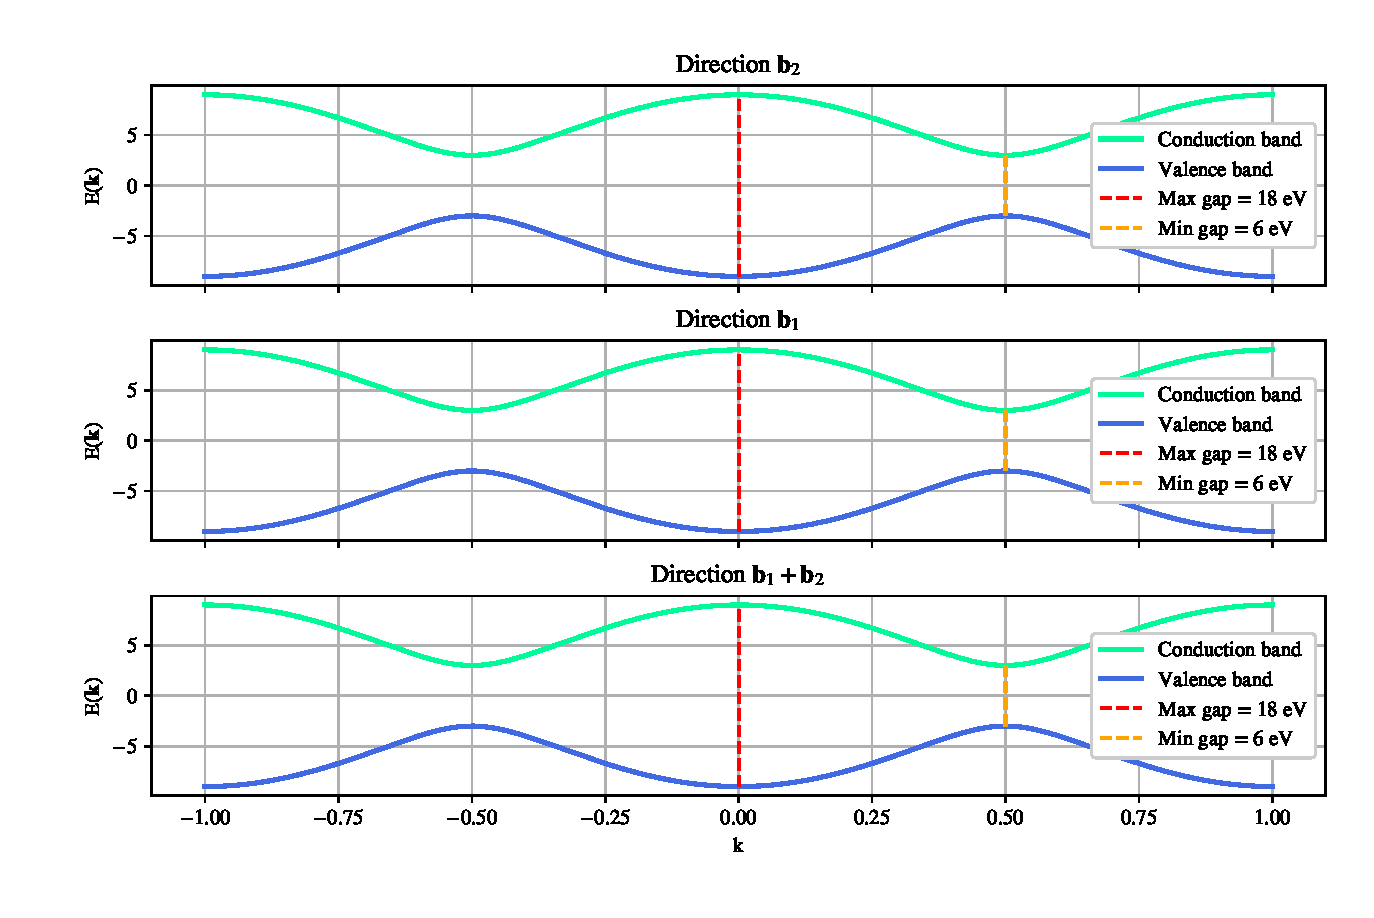
\includegraphics[scale=0.7]{Ek.eps}
    \caption{Energy dispersion relation function in a 2D graphene sheet. The first plot 
    corresponds to the direction $\ve b_1$, the second to the direction $\ve b_2$ and the third to the direction $\ve b_1 + \ve b_2$.}
    \label{fig:E_k}
\end{figure}
\subsubsection*{(b)}
The gradient of the energy is 
\begin{equation*}
    \vec \nabla_k E(\ve k) = \left(
        -6a\cos\left(\frac{\sqrt{3}k_ya}{2}\right)
        \sin\left(\frac{3k_xa}{2}\right), \ 
        -2\sqrt{3}a\sin\left(\frac{\sqrt{3}k_ya}{2}\right) 
        -4\sqrt{3}a\cos\left(\frac{3k_xa}{2}\right) 
        \sin\left(\frac{\sqrt{3}k_ya}{2}\right) 
    \right)
\end{equation*}
hence by taking the scalar product with $\ve b_1 = \frac{2\pi}{a}(\frac{1}{3}, \frac{1}{\sqrt{3}})$ and inserting into \ref{eq:effective_mass_der1} one gets an expression for the mass along 
$\ve b_1$ which is plotted in figure \ref{fig:m_eff}.
\begin{figure}
    \centering 
    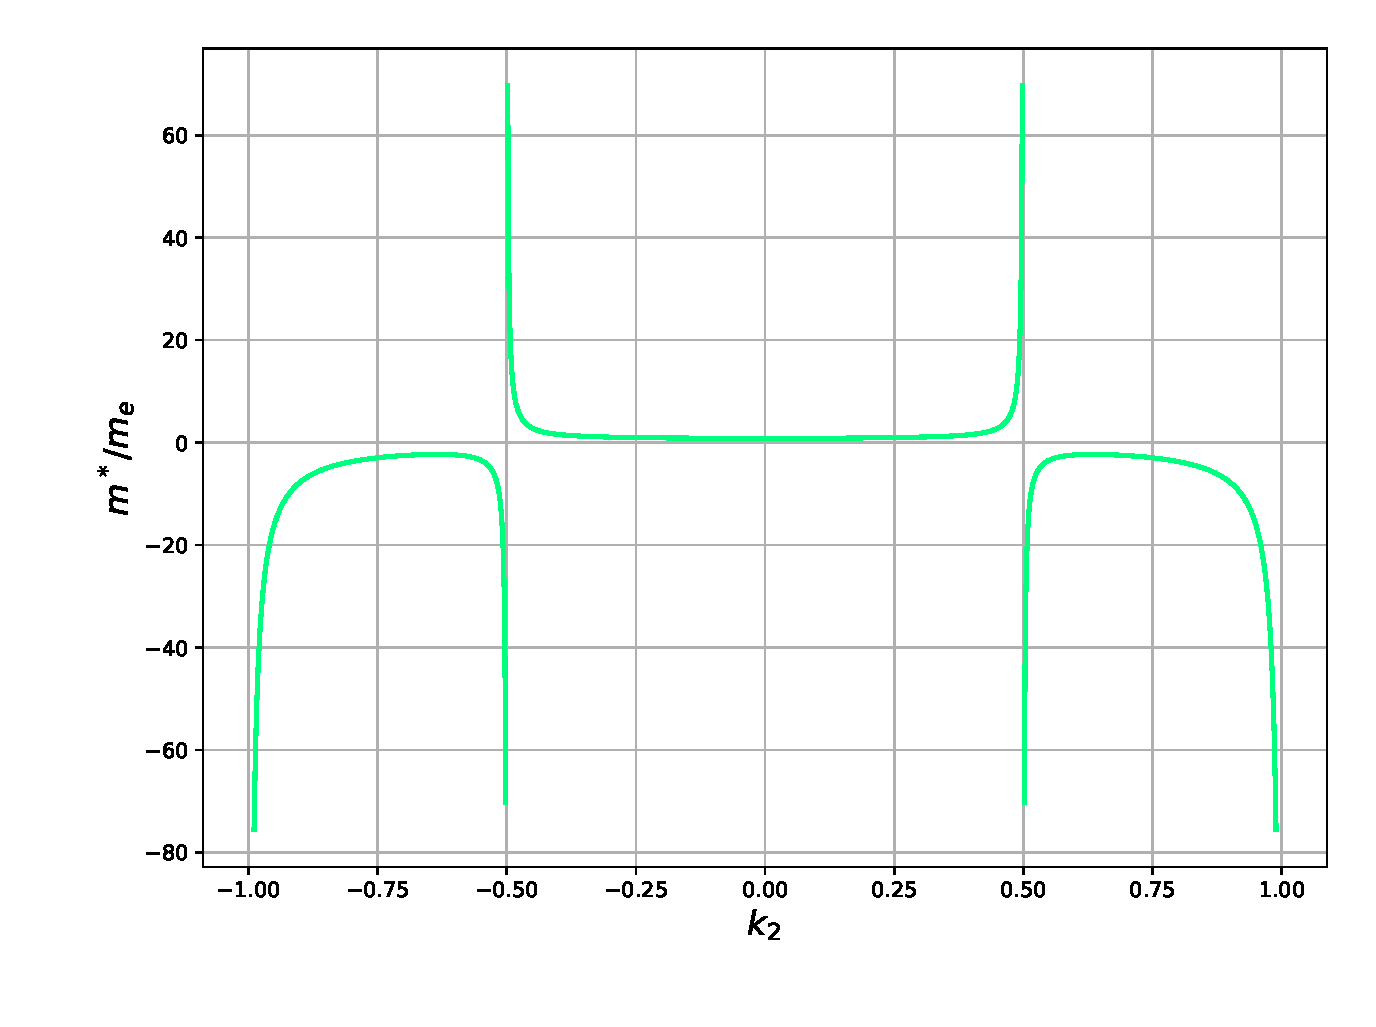
\includegraphics[scale=0.5]{meff.eps}
    \caption{Effective electron mass in a 2D graphene sheet along direction [01] of the Brillouin zone}
    \label{fig:m_eff}
\end{figure}
Let us take again expression \ref{eq:effective_mass_der1} along $k_x$. In the limit $k_x,k_y \to 0$ the expression asymptotically approaches
\begin{equation*}
    m_{e, \ve k_x}^* \approx \hbar^2 \frac{2}{3a^2t} = 0.839 \, m_e
\end{equation*}
The result coincides numericaly with the one obtained via the second derivative approach
\begin{equation*}
    m_{e, \ve k_x}^* = \hbar^2\left(\frac{\partial^2 E(\ve k)}{\partial k_x^2}\right)^{-1} = \hbar^2\left(\frac{\partial^2 E(\ve k)}{\partial k_y^2}\right)^{-1}
\end{equation*}
Note, however, that this last expression holds only in a neighbourhood of the extremal point of the bands, while equation \ref{eq:effective_mass_der1} is a more general expression. \\
Note also that at the edge of the Brillouin zone the mass diverges!

\newpage

\section*{Exercise 2}
The electrons' density of states in the conduction band is 
\begin{equation*}
    D_{e}(\boldsymbol{\epsilon})=\frac{1}{2 \pi^{2}}\left(\frac{2 m_{e}}{\hbar^{2}}\right)^{3 / 2}\left(\boldsymbol{\epsilon}-E_{c}\right)^{1 / 2}
\end{equation*}
hence the number of intrinsic carriers in the conduction band at temperature $T$ can be calculated as 
\begin{gather*}
    n(T) = \int_{E_C}^{+\infty} D_e(\epsilon) \ f_{FD}(\epsilon) \ d\epsilon = \\
    = \frac{1}{2 \pi^{2}}\left(\frac{2 m_{e}}{\hbar^{2}}\right)^{3 / 2}\int_{E_C}^{+\infty} \left(\boldsymbol{\epsilon}-E_{c}\right)^{1 / 2} \ \frac{1}{1+\exp\left((\epsilon - E_f)/k_BT\right)} \ d\epsilon \approx \\ 
    \approx \frac{1}{2 \pi^{2}}\left(\frac{2 m_{e}}{\hbar^{2}}\right)^{3 / 2}\int_{E_C}^{+\infty} \left(\boldsymbol{\epsilon}-E_{c}\right)^{1 / 2} \ \exp\left((\epsilon-E_f)/k_BT\right) \ d\epsilon = \\
    = 2 \left(\frac{m_ek_BT}{2\pi\hbar^2}\right)^{3/2} \, \exp\left(\frac{E_f-E_C}{k_BT}\right) \equiv N_C \exp\left(\frac{E_f-E_C}{k_BT}\right)
\end{gather*} 
In a similar way the concentration of holes is 
\begin{gather*}
    p(T) = \int_{E_C}^{+\infty} D_e(\epsilon) \ \left(1-f_{FD}(\epsilon)\right) \ d\epsilon = \\
    = 2 \left(\frac{m_hk_BT}{2\pi\hbar^2}\right)^{3/2} \, \exp\left(\frac{E_V-E_f}{k_BT}\right) \equiv N_V \exp\left(\frac{E_V-E_f}{k_BT}\right)
\end{gather*}
and one can notice that  
\begin{equation*}
    p(T) \, n(T) = N_CN_V \exp\left(\frac{E_V-E_C}{k_bT}\right) \equiv n_i^2(T)
\end{equation*}
For intrinsic carriers one has that $n(T)=p(T)=n_i(T)$, while in general one can rewrite $n(T)$ and $p(T)$ as
\begin{gather}
    n(T) = n_i(T)\exp\left(\frac{E_f-E_i}{k_BT}\right) 
    \label{eq:n(T)} \\
    p(T) = n_i(T)\exp\left(\frac{E_i-E_f}{k_BT}\right)
\end{gather}
Expression \ref{eq:n(T)} give the number of conduction electrons as a function of temperature. To obtain
the expression of the fermi energy it is convenient to make use of the \emph{Mass-Action law}. In a doped semiconductor the Mass-Action law estabilishes that
\begin{equation*}
    N_D^+ + p = N_A^- + n
\end{equation*}
or, in the case of $N_A^- = 0$ as in this case 
\begin{equation}
    N_D^+ + p = n
    \label{eq:charge_balance}
\end{equation}
Let us call $E_D$ the energy difference between the donors's energy level and the lower limit of the conduction band.
The number of ionized donors at temperature $T$ is given by
\begin{equation*}
    N_D^+ = N_D \left(1 - \frac{1}{1+\frac{1}{2}\exp\left(\frac{E_D-E_f}{k_BT}\right)}\right) = \frac{N_D}{1 + 2\exp\left(\frac{E_f-E_D}{k_BT}\right)}
\end{equation*}
where the factor $1/2$ in the Fermi-Dirac distribution takes account of the spin degeneracy. \\
Equation \ref{eq:charge_balance} becomes 
\begin{equation*}
    n_i(T)\exp\left(\frac{E_f-E_i}{k_BT}\right) + \frac{N_D}{1 + 2\exp\left(\frac{E_f-E_D}{k_BT}\right)} - n_i(T)\exp\left(\frac{E_i-E_f}{k_BT}\right) = 0
\end{equation*}
or 
\begin{equation*}
    2 \, n_i(T) \, \sinh\left(\frac{E_f-E_i}{k_BT}\right) + \frac{N_D}{1 + 2\exp\left(\frac{E_f-E_D}{k_BT}\right)} = 0
\end{equation*}
This equation can be solved numerically for $E_f$, the value of which can be popped into \ref{eq:n(T)} to obtain the concentration of conducting electrons.
The energy $E_i$, namely the \emph{intrinsic Fermi energy}, is a function of the effective mass of the electrons and holes in the semiconductor. It can be easilly calculated
in the intrinsic case by imposing $n(T) = p(T)$, that is 
\begin{equation*}
    N_C e^{\frac{E_{f}-E_C}{k_B T}} = N_V e^{\frac{E_V- E_{f}}{k_B T}}
\end{equation*}
After some algebra one gets that 
\begin{equation*}
    E_i = \frac{1}{2}E_g + \frac{3}{4}k_BT\log\left(\frac{m_h^*}{m_e^*}\right)
\end{equation*}
where $E_g = E_C - E_D$ is the energy gap, $m_h^*$ and $m_e^*$ are the effective masses of holes and electrons. \\
Both $E_F$ and $E_i$ as functions of temperature are reported in figure \ref{fig:efei}. Here I report the values of the parameters that I used in the analysis
\begin{center}\begin{gather*}
    m_e^* = 1.08 \, m_e \qquad m_h^* = 0.56 \, m_e \\
    E_V = \SI{0}{\electronvolt} \qquad E_c = E_g = \SI{1.1}{eV} \\
    E_D = \SI{1.055}{\electronvolt} \qquad N_d = 10^{17} \small{\frac{P}{cm^3}} 
\end{gather*}\end{center}

\begin{figure}[h]
    \centering 
    \includegraphics[scale=0.6]{efei.eps}
    \caption{Fermi energy and intrinsic fermi energy in a silicon semiconductor with doping concentration $10^{17} P/cm^3$}
    \label{fig:efei}
\end{figure}

\subsubsection*{Low temperature (freeze-out region)}
In the regime of low temperature, in first approximation, all the electrons in the conduction band come from ionized impurities since they are higher in energy than the electrons in the valence band.
Hence, for low $T$:
\begin{equation*}
    n(T) \approx N_D^+(T) = \frac{N_D}{1 + 2\exp\left(\frac{E_f-E_D}{k_BT}\right)}
\end{equation*}
The approximated expression for the fermi energy can be obtained by imposing 
\begin{equation*}
    n(T) \approx N_D^+(T) \qquad \longleftrightarrow \qquad \frac{N_D}{1 + 2\exp\left(\frac{E_f-E_D}{k_BT}\right)} = N_C \exp\left(\frac{E_f-E_C}{k_BT}\right)
\end{equation*}
and yields
\begin{equation*}
    E_{f}=\frac{E_{C}+E_{D}}{2}+\frac{k T}{2}\ln\left(\frac{N_D}{2N_C}\right)
\end{equation*}
\subsubsection*{Medium temperature (extrinsic region)}
For medium temperature all the impurities are ionized and only few electrons are excited from the valence band, hence 
\begin{equation*}
    n(T) \approx N_D
\end{equation*}
\subsubsection*{High temperature (intrinsic region)}
Finally, for high temperature, impurities and intrinsic donors both contribute to the number of electrons, but the number of intrinsic carries is normally way greater than 
the number of impurities addded, hence 
\begin{equation*}
    n(T) \approx n_i(T) = N_C \exp\left(\frac{E_f-E_C}{k_BT}\right)
\end{equation*}
The fermi energy is approximately equal to the intrinsic fermi energy, since we are neglecting the donors' contribution.
\vspace{10pt}
All the approximated analytical results together with the numerical one are reported in figure \ref{fig:concentration}

\begin{figure}[h]
    \centering
    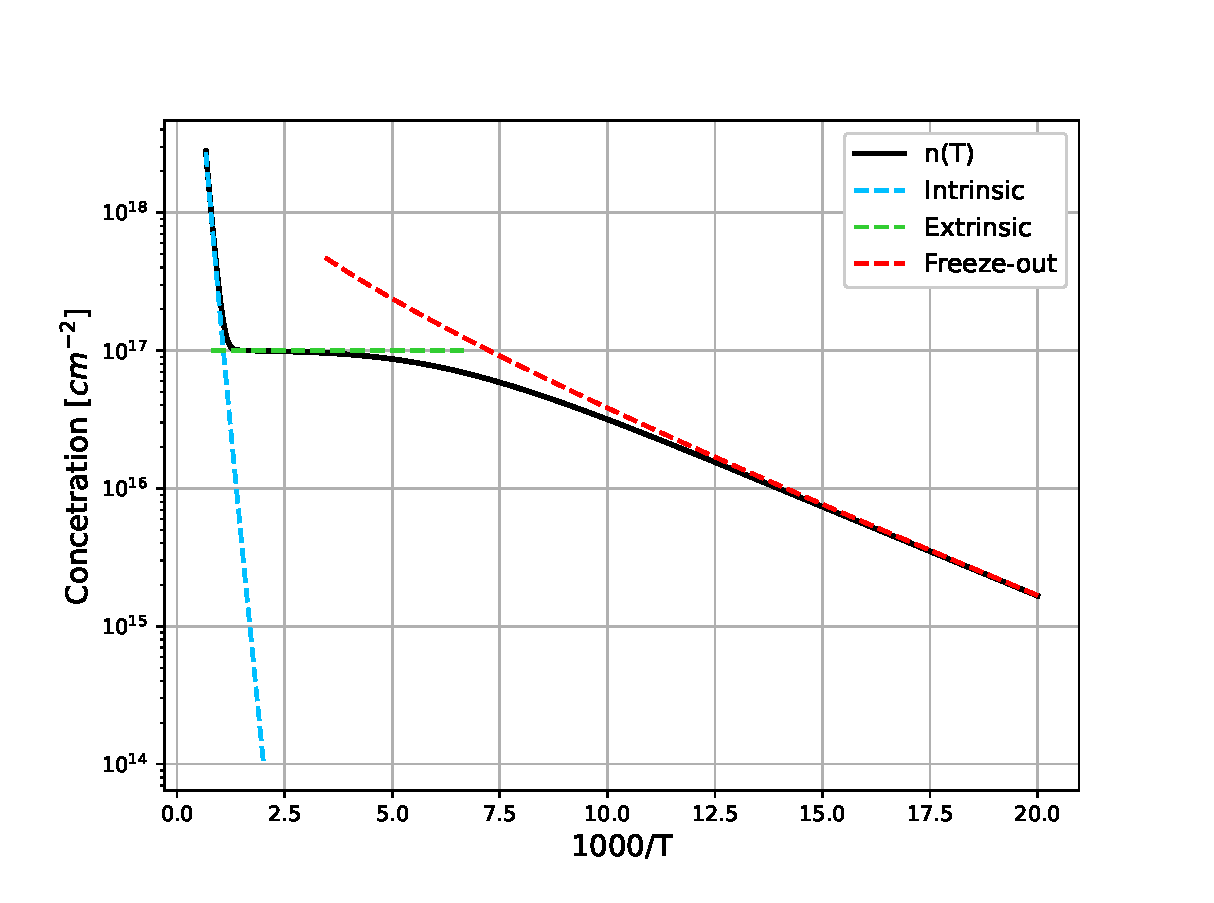
\includegraphics[scale=0.6]{concentration.eps}
    \caption{Carrier concentration in a silicon semiconductor with doping concentration $10^{17} P/cm^3$.}
    \label{fig:concentration}
\end{figure}



\end{document}